% !TeX TXS-program:compile = txs:///pdflatex/[--shell-escape]

\documentclass[11pt, letterpaper]{article}

\usepackage{minted}
\usepackage[utf8]{inputenc}
\usepackage[T1]{fontenc}
\usepackage{lmodern}
\usepackage{graphicx}
\usepackage{longtable}
\usepackage{wrapfig}
\usepackage{rotating}
\usepackage{amsmath}
\usepackage{textcomp}
\usepackage{amssymb}
\usepackage{hyperref}
\usepackage[round]{natbib}
\usepackage{subcaption}


\title{\bfseries Tarea}
\author{Ángel García Báez}
\date{\today}
\setcounter{tocdepth}{3} 

\begin{document}
	
	% Página de presentación
	\begin{titlepage}
		\centering
		
\includegraphics[width=0.2\textwidth]{logo.png}\par
		\vspace{1cm}
		{\LARGE \bfseries Universidad Veracruzana \par}
		\vspace{1cm}
		{\Large Maestría en Inteligencia Artificial\par}
		\vspace{3cm}
		{\LARGE \bfseries Visión por Computadora \par}
		\vspace{1cm}
		{\Large \bfseries Tarea 8. Aplicación de un proceso de registro sobre 1520 imágenes respecto a una de referencia en MATLAB. \par}
		\vfill
		{\Large \textit{Ángel García Báez}\par}
		\vspace{1cm}
		{\Large Profesor: Dr. Héctor Acosta Mesa \par}
		\vfill
		{\Large \today \par}
	\end{titlepage}
	
	% Página exclusiva para la tabla de contenidos
	\newpage
	\tableofcontents
	\newpage
	
% Sección para el problema 1
\section{Objetivo de la práctica}

Para la presente practica, se cuenta con un conjunto de 1520 imágenes, donde cada una de ellas tiene asociada una matriz extra de puntos de referencia de tamaño $20 \times 2$. Se desea realizar un proceso de registro usando los puntos de referencia y tomando en cuenta la primer imagen del conjunto junto con sus puntos:


\begin{figure}[h!]
	\centering
	\begin{minipage}{0.4\textwidth}
		\centering
		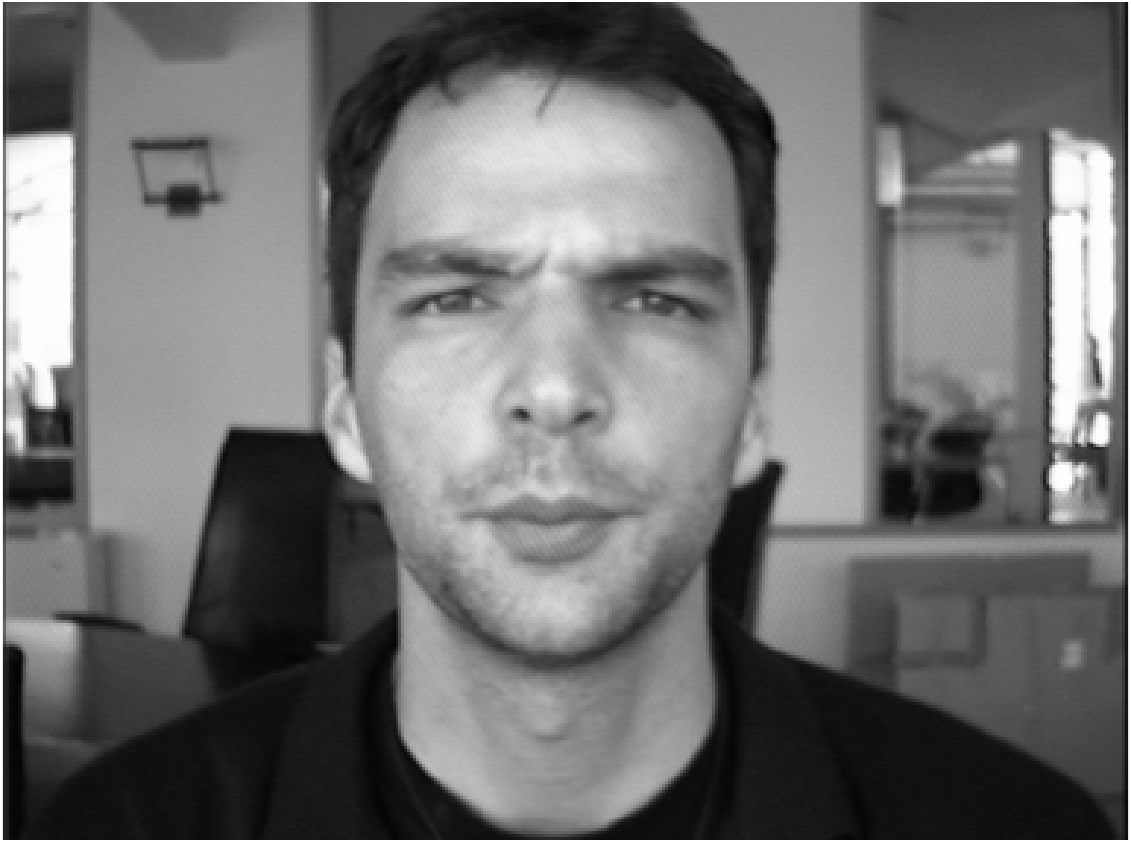
\includegraphics[width=\textwidth]{IMG/R0.png}
		\caption*{(a) Imagen 1 del conjunto.}
	\end{minipage}\hfill
	\begin{minipage}{0.4\textwidth}
		\centering
		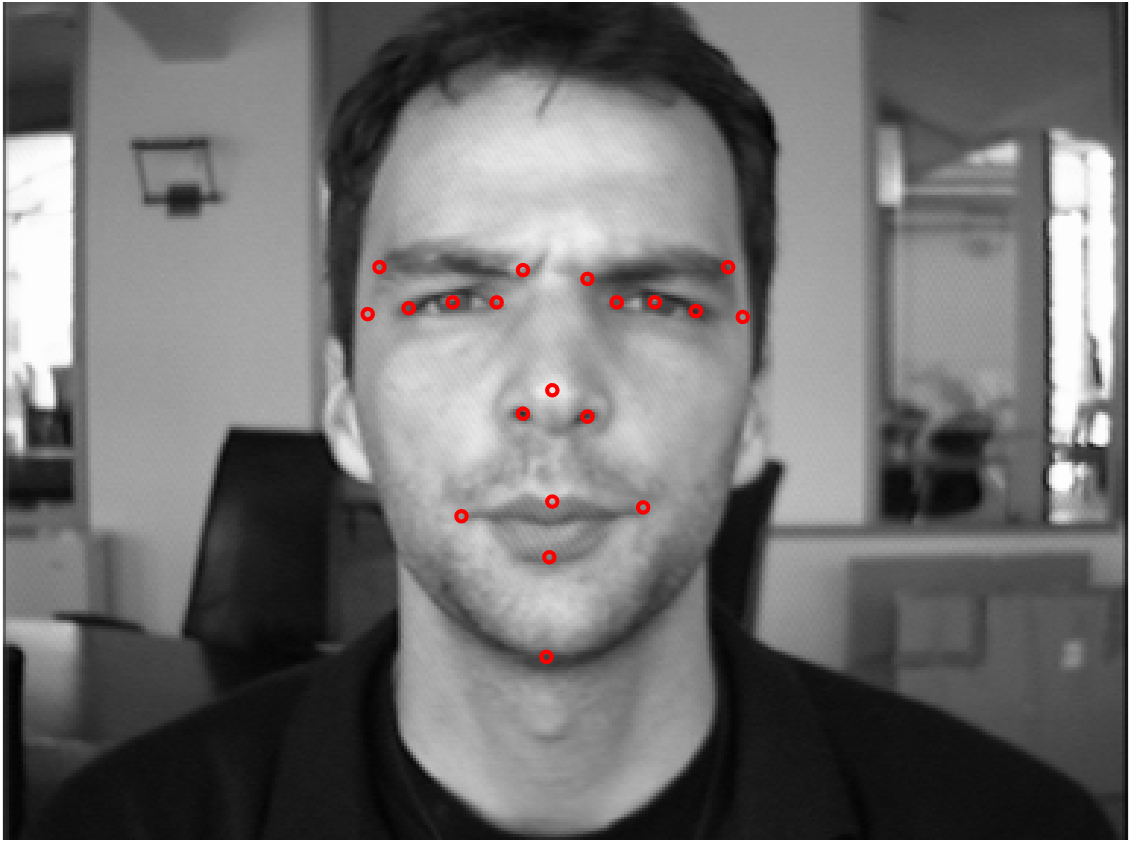
\includegraphics[width=\textwidth]{IMG/R1.png}
		\caption*{(b) Imagen 1 con sus puntos de referencia.}
	\end{minipage}
	\caption{Imagen y puntos de referencia.}
	\label{fig:r0_r1}
\end{figure}

Para ello, se pide hacer lo siguiente:

\begin{itemize}
	\item Mostrar el mapa de distribución de puntos antes del registro de las imagenes
	\item Registrar las 1520 imágenes tomando como referencia la primer imagen.
	\item Calcular el error cuadratico medio y seleccionar a las 99 que más se parezcan a la de referencia (es decir, que tengan un menor ECM)
	\item Mostrar el mapa de distribución de puntos de las 100 imagenes registradas con menor ECM.	
	
\end{itemize}




	
\newpage
	
\section{Metodología}

De acuerdo con \cite{gonzalez2018digital}, el proceso de registro en imágenes, es el proceso de alinear dos o más imágenes que pueden presentar deformaciones o estar desfasadas espacialmente por algún tipo de rotación, traslación o escala para que sus elementos de interés (boca, nariz ojos, etc...) coincidan en la misma posición. .

Para realizar este proceso, es fundamental hacer la selección de puntos de control (o Landmarks), regularmente se suelen marcar zonas clave de interés (en el caso de trabajar con rostros) como la boca, los ojos, la nariz. Para ello es necesario obtener dichos puntos de la imagen que sera usada como referencia a la cual se quieren hacer coincidir los puntos y los puntos de la imagen que se desea registrar.

Se pueden denotar como 

\begin{itemize}
\item $p_i \in R^2$: Son los puntos de la imagen a registrar.
\item $q_i \in R^2$: Son los puntos de la imagen de referencia.
\end{itemize}

El siguiente paso, es encontrar una transformación $T$ que permita mapear los puntos de registro respecto a los puntos de la imagen de referencia tal que:

$$T(p_i)\sim q_i $$

Una gama de posibles transformaciones ya fue mencionada en la tarea 7, por lo que no se hace mayor énfasis en esta parte.

Para el caso particular de esta aplicación, se desea obtener una transformación afín homogénea que permita hacer el registro.

$$
\begin{bmatrix}
	x' \\
	y' \\
	1
\end{bmatrix}
=
\underbrace{
	\begin{bmatrix}
		a_{11} & a_{12} & t_x \\
		a_{21} & a_{22} & t_y \\
		0 & 0 & 1
	\end{bmatrix}
}_{\text{Matriz de transformación homogénea}}
\cdot
\begin{bmatrix}
	x \\
	y \\
	1
\end{bmatrix}
$$

Donde:

\begin{itemize}
	\item $a_{11}, a_{12}, a_{21}, a_{22}$ codifican rotación, escala y cizalla.
	\item $t_x, t_y$ representan la traslación en los ejes $x$ e $y$, respectivamente.
	\item El vector $\begin{bmatrix} x \\ y \\ 1 \end{bmatrix}$ es el punto original en coordenadas homogéneas.
\end{itemize}

Una vez encontrada  dicha transformación $T$, se procede a aplicar la transformación sobre los puntos de control de la imagen a la que se le quiere hacer el registro.

Hasta aquí quedaría el proceso, pero aun falta evaluar que tan bueno fue dicho ajuste mediante la transformación, para ello se evaluá mediante el error cuadrático medio entre los puntos con la transformación afín y los puntos de referencia como sigue:

$$ECM = \frac{1}{N}\sum^N_{i = 1}{||T(p_i) -q_i||^2}$$

Donde: 

\begin{itemize}
	\item $ECM$: Error Cuadrático Medio.
	\item $N$: Número total de puntos.
	\item $p_i$: Punto $i$ del conjunto original.
	\item $T(p_i)$: Punto $p_i$ después de aplicar la transformación $T$.
	\item $q_i$: Punto $i$ del conjunto de referencia.
	\item $\|\cdot\|$: Norma euclidiana (distancia entre puntos).
\end{itemize}

Una vez definidos los elementos necesarios, a continuación se explican los pasos a seguir para la obtención de los resultados:

\begin{itemize}
	\item Primero se obtuvo el gráfico de los 1520 conjuntos de puntos correspondientes a sus imágenes y se graficaron.
	
	\item Segundo, se hizo el registro de cada uno de los 1520 conjuntos de puntos respecto a la imagen 1 y se graficaron. 
	
	\item Tercero, se obtuvo el ERM de cada conjunto de puntos transformado respecto al conjunto de la imagen 1 para evaluar que tan bueno fue el ajuste. Se hizo el histograma de la distribución de los errores cuadráticos medios y se ordenaron de menor a mayor.
	
	\item Finalmente, se obtuvieron unicamente los 100 conjuntos de puntos transformados que presentaron el error cuadrático más pequeño y se graficaron.
	
\end{itemize}



\newpage
	
\section{Resultados}

\subsection{Distribución antes del registro}

\begin{figure}[h!]
	\centering
	\begin{minipage}{0.4\textwidth}
		\centering
		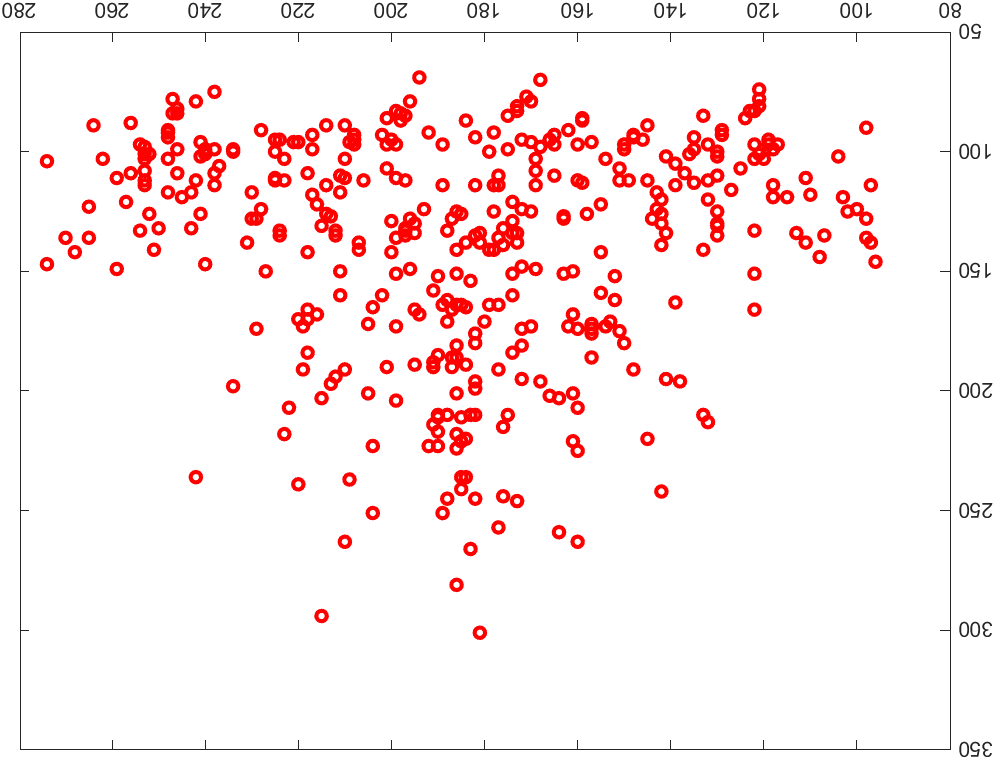
\includegraphics[width=\textwidth]{IMG/R2.png}
		\caption*{(a) Distribución de los puntos.}
	\end{minipage}\hfill
	\begin{minipage}{0.4\textwidth}
		\centering
		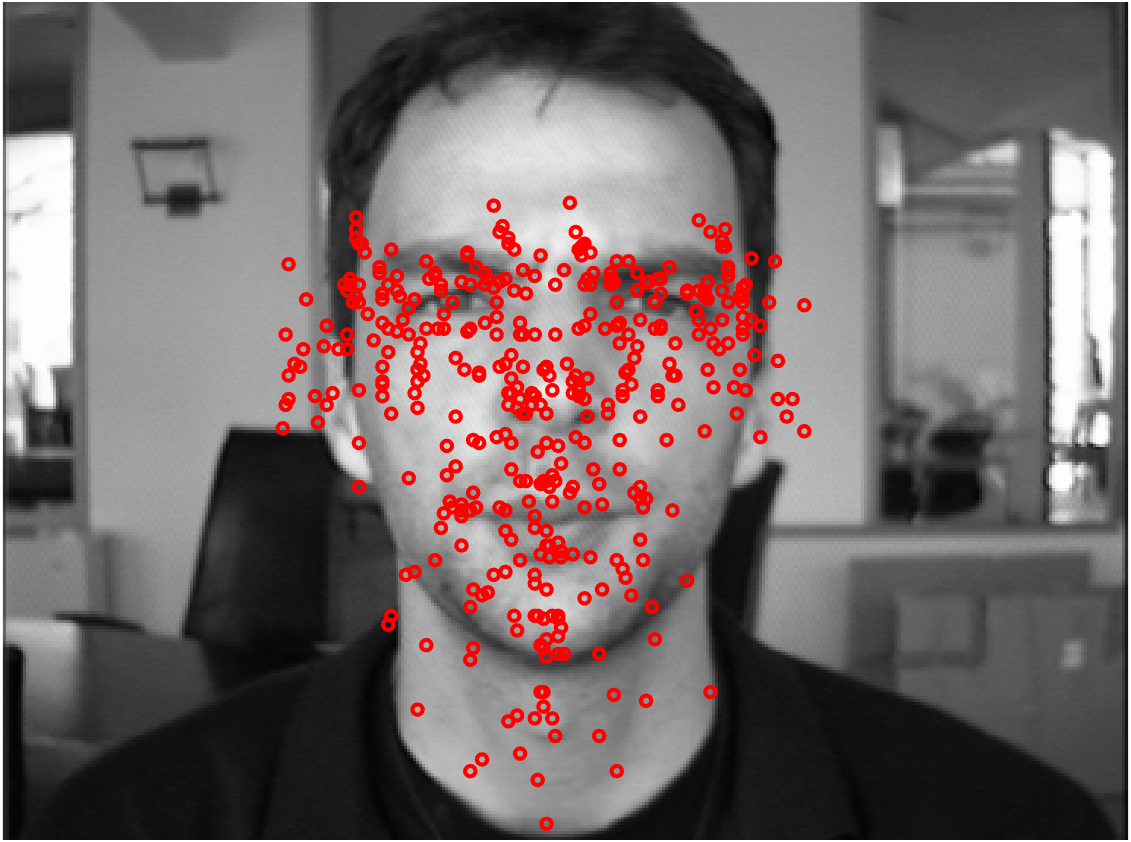
\includegraphics[width=\textwidth]{IMG/R3.png}
		\caption*{(b) Imagen con la distribución de los puntos.}
	\end{minipage}
	\caption{Imagen y puntos de referencia.}
	\label{fig:f2}
\end{figure}

El gráfico de distribución de los puntos muestra como se distribuyen los puntos de los 1520 conjuntos alrededor de la imagen de referencia, se observa como hay puntos que cubren todos los alrededores de las zonas clave (ojos, nariz y boca) de tal forma que se "desbordan" respecto a la imagen de referencia.


\newpage

\subsection{Distribución después del registro}

\begin{figure}[h!]
	\centering
	\begin{minipage}{0.4\textwidth}
		\centering
		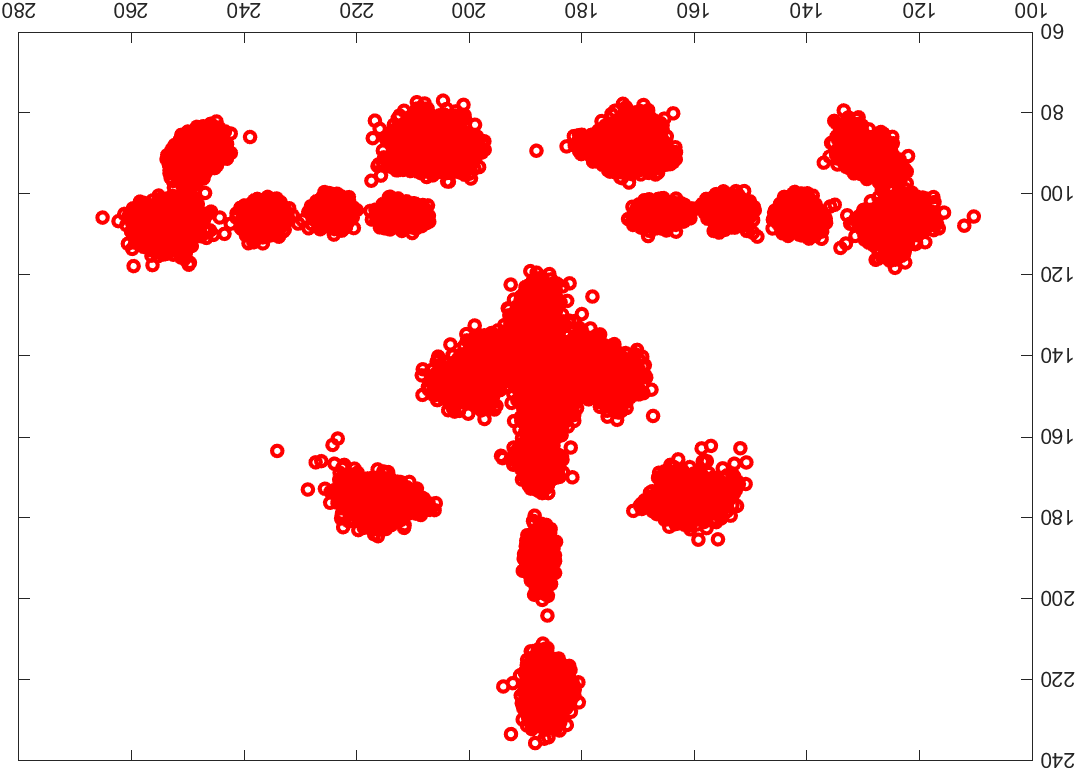
\includegraphics[width=\textwidth]{IMG/R5.png}
		\caption*{(a) Distribución de los puntos despues del registro.}
	\end{minipage}\hfill
	\begin{minipage}{0.4\textwidth}
		\centering
		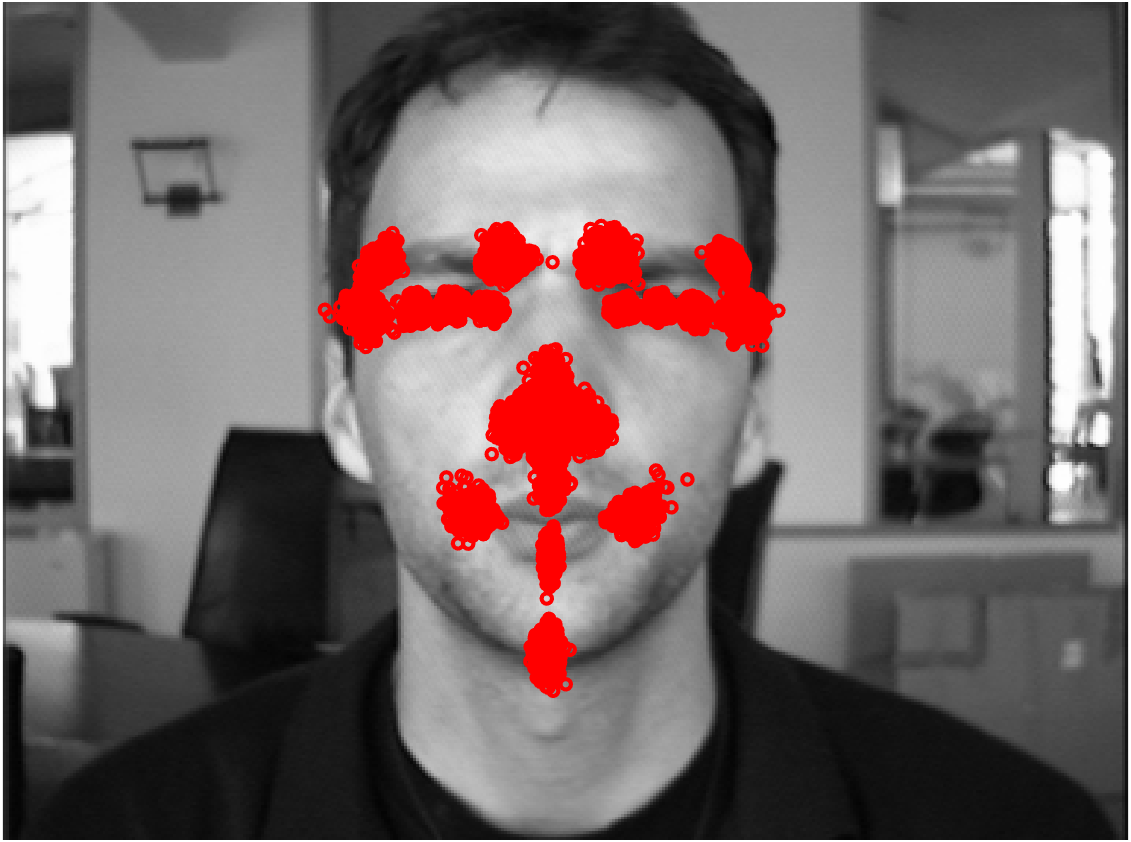
\includegraphics[width=\textwidth]{IMG/R6.png}
		\caption*{(b) Imagen con la distribución de los puntos después del registro.}
	\end{minipage}
	\caption{Imagen y puntos de referencia.}
	\label{fig:f3}
\end{figure}

Tras el proceso de registro, se observa como los puntos transformados se agrupan de forma que ahora sí están siendo compactados lo más posible dentro de las zonas de interés de la primer imagen, es decir, visualmente los puntos no se están desbordando de las zonas de interés, por lo que el proceso de registro fue exitoso.


\newpage

\subsection{Selección de los ERM}

\begin{figure}[h!]
	\centering
	\begin{minipage}{0.5\textwidth}
		\centering
		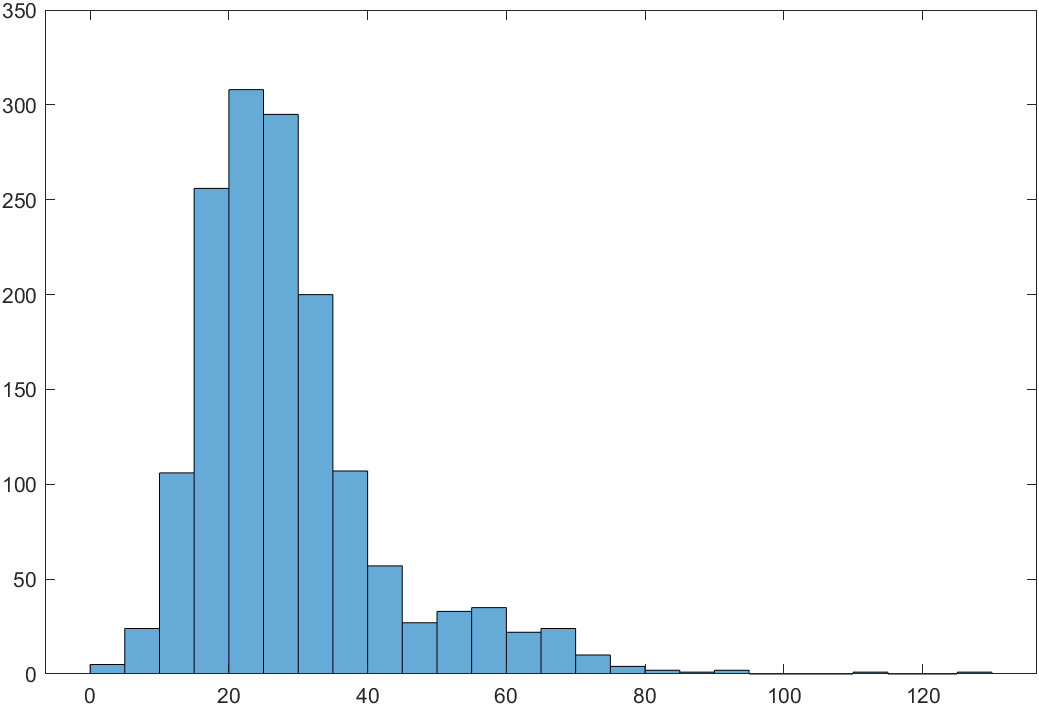
\includegraphics[width=\textwidth]{IMG/R4.png}
		\caption*{(a) Histograma de los errores cuadráticos medios.}
	\end{minipage}\hfill
	\begin{minipage}{0.25\textwidth}
		\centering
		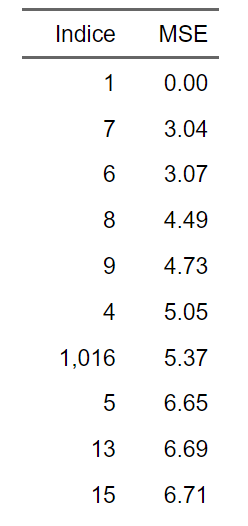
\includegraphics[width=\textwidth]{IMG/R4.1.png}
		\caption*{(b) Muestra de los mejores ordenados por ECM .}
	\end{minipage}
	\caption{Imagen y puntos de referencia.}
	\label{fig:f4}
\end{figure}

El histograma muestra como una parte considerable de los conjuntos de puntos se encuentran mayormente entre valores de 20 y 40 unidades. 

La tabla de los ECM ordenados muestra como los puntos de referencia registrados consigo mismos, dan un error de 0, siendo que el segundo mejor conjunto reporta un valor del ECM = 3.04.


\newpage

\subsection{Distribución con los primeros 100 mejores}

\begin{figure}[h!]
	\centering
	\begin{minipage}{0.4\textwidth}
		\centering
		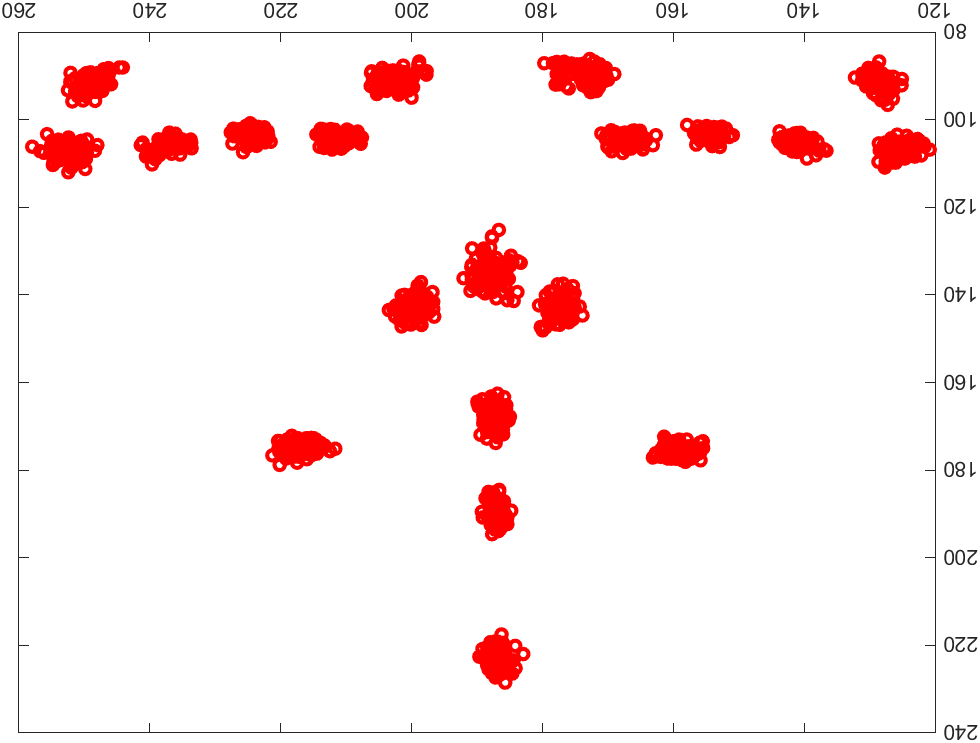
\includegraphics[width=\textwidth]{IMG/R7.png}
		\caption*{(a) Distribución de los 100 mejores puntos después del registro.}
	\end{minipage}\hfill
	\begin{minipage}{0.4\textwidth}
		\centering
		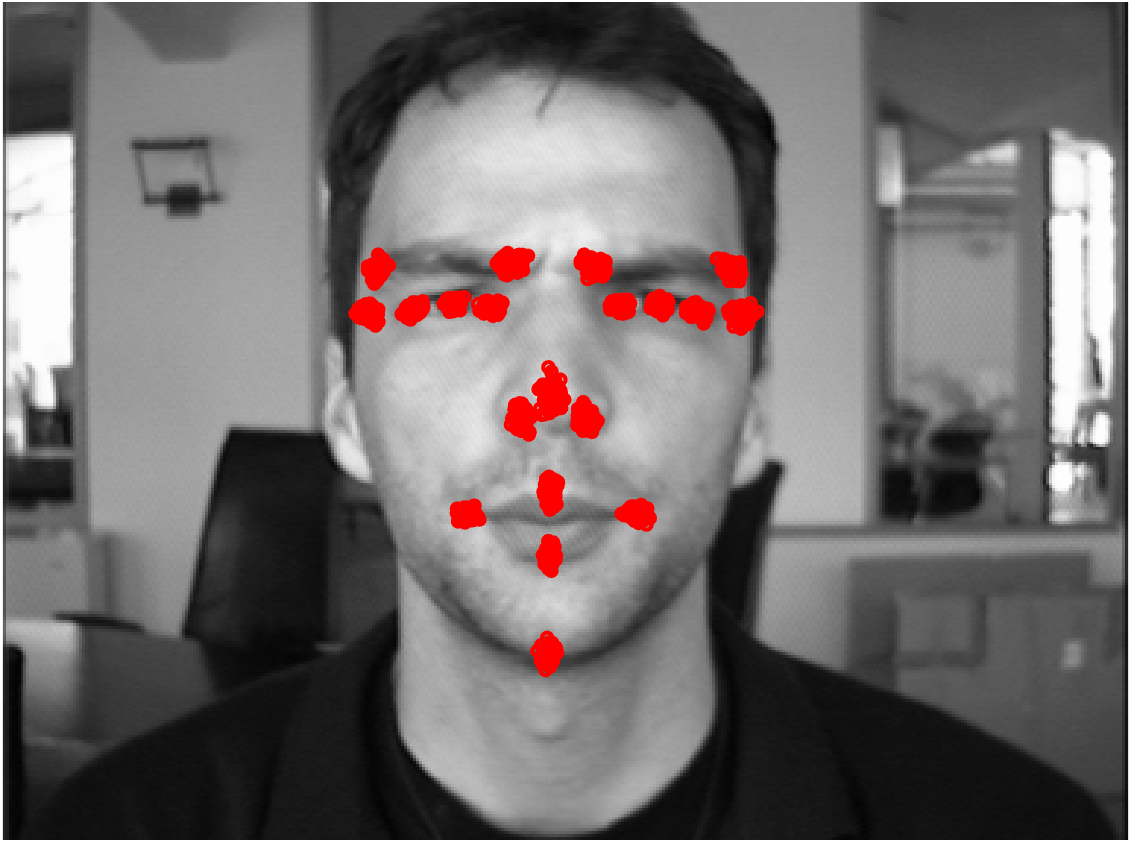
\includegraphics[width=\textwidth]{IMG/R8.png}
		\caption*{(b) Imagen con la distribución de los 100 mejores puntos después del registro.}
	\end{minipage}
	\caption{Imagen y puntos de referencia.}
	\label{fig:f5}
\end{figure}

Al escoger unicamente a los 100 con menor error cuadrático medio, se observa como los conjuntos de puntos marcan de forma muy compacta la zona alrededor de los puntos de referencia, siendo más notable esto en la zona de la nariz, donde son muy puntuales las acumulaciones en comparación con la imagen con todos los puntos registrados en donde se ve como los puntos se expanden por toda la nariz.

\newpage
	
\section{Conclusiones}

Tras la implementación y evaluación del proceso de registro, se puede concluir que el proceso cumple con su trabajo, ademas que muestra lo importante que es evaluar que tan bueno fue dicho proceso de registro para el ajuste y estandarización de las imágenes mediante puntos de control.	
	

\newpage

	
\section{Referencias}  % Sección numerada de referencias
\bibliographystyle{apalike}  % Estilo de citas (puedes cambiarlo)
\bibliography{Biblio}        % Nombre del archivo BibTeX (sin extensión)

\newpage
	
\section{Anexos}	
\subsection{Implementación del proceso de registro y exploración en MATLAB}
\begin{minted}[linenos,firstnumber=1]{matlab}
%% Cargar los datos de los puntos %%
ruta1 = "C:\\Users\\Angel\\Desktop\\BioID1520 1\\data_points.mat";
data = load(ruta1);
points = data.data;

%% Cara de referencia 
ruta2 = "C:\\Users\\Angel\\Desktop\\BioID1520 1\\Im_Faces\\BioID_0001.pgm";
face = imread(ruta2);
NI = 1520;
% Extraer los puntos de la primera imagen
puntos1 = squeeze(points(1, :, :))'; % tamaño: 20 × 2


%% Registrar respecto a la primer imagen %%
% Proceso de registro %%
registro = zeros(NI, 2 , 20);
for m = 1:NI    
% Convertir los puntos i-esimos a matriz
coords = squeeze(points(m, :, :))';    
% Obtener la transformación afín homogenea
tform = fitgeotrans(coords, puntos1, 'affine');
T = tform.T;
% Obtención del registro
for i = 1:20
[x2, y2] = transformPointsForward(tform, ...
coords(i,1), coords(i,2));
% Acomodar las nuevas coordenadas 
registro(m, 1, i) = x2;
registro(m, 2, i) = y2;
end
end



%% Obtener el ERM %%
errores = zeros(NI,1);
for m = 1:NI
% Extraer los puntos registrados 
puntos_m = squeeze(registro(m, :, :))'; % 20x2
% Calcular la diferencia entre cada par de puntos
dif = puntos_m - puntos1;
% Calcular el error cuadratico medio %
errores(m) = mean(sum((dif).^2,2));
end

%% Ordenar los errores de menor a mayor %%
[errores_ordenados, indices_ordenados] = sort(errores);

%% Seleccionar las 99 mejores imágenes %%
mejores99 = indices_ordenados(1:100);

%% Proyectando resultados %%

%% Proyectar la imagen con sus puntos %%
imshow(face);
hold on; % Mantener la imagen para dibujar encima
% Dibujar los puntos
plot(puntos1(:,1), puntos1(:,2), 'ro', 'MarkerSize', 5, 'LineWidth', 2);
hold off;

%% Distribución de todos los puntos %%
for i = 1:size(puntos1,1)
% Pasar por cada punto y extraer sus coordenadas
puntosi = squeeze(points(i, :, :))'; % tamaño: 20 × 2
% Armar un gráfico con los puntos 
plot(puntosi(:,1), puntosi(:,2), 'ro', ...
'MarkerSize', 5, 'LineWidth', 2);
hold on; % Mantener la imagen para dibujar encima
end

%% Distribución de todos los puntos sobre la imagen %%
imshow(face);
hold on; % Mantener la imagen para dibujar encima
for i = 1:size(puntos1,1)
% Pasar por cada punto y extraer sus coordenadas
puntosi = squeeze(points(i, :, :))'; % tamaño: 20 × 2
% Armar un gráfico con los puntos 
plot(puntosi(:,1), puntosi(:,2), 'ro', ...
'MarkerSize', 5, 'LineWidth', 2);
hold on; % Mantener la imagen para dibujar encima
end

%% Histograma de los errores %%
histogram(errores)

%% Distribución de los puntos registrados %%
for i = 1:NI
% Pasar por cada punto y extraer sus coordenadas
puntosi = squeeze(registro(i, :, :))'; % tamaño: 20 × 2
% Armar un gráfico con los puntos 
plot(puntosi(:,1), puntosi(:,2), 'ro', ...
'MarkerSize', 5, 'LineWidth', 2);
hold on; % Mantener la imagen para dibujar encima
end

%% Distribución de los puntos registrados sobre la imagen %%
imshow(face);
hold on; % Mantener la imagen para dibujar encima
for i = 1:NI
% Pasar por cada punto y extraer sus coordenadas
puntosi = squeeze(registro(i, :, :))'; % tamaño: 20 × 2
% Armar un gráfico con los puntos 
plot(puntosi(:,1), puntosi(:,2), 'ro', ...
'MarkerSize', 5, 'LineWidth', 2);
hold on; % Mantener la imagen para dibujar encima
end

%% Distribución de los mejores 100 %%
for i = 1:100
% Mejores
mj = mejores99;
% Pasar por cada punto y extraer sus coordenadas
puntosi = squeeze(registro(mj(i), :, :))'; % tamaño: 20 × 2
% Armar un gráfico con los puntos 
plot(puntosi(:,1), puntosi(:,2), 'ro', ...
'MarkerSize', 5, 'LineWidth', 2);
hold on; % Mantener la imagen para dibujar encima
end

%% Distribución de los mejores 100  sobre la imagen %%
imshow(face);
hold on; % Mantener la imagen para dibujar encima
for i = 1:100
% Mejores
mj = mejores99;
% Pasar por cada punto y extraer sus coordenadas
puntosi = squeeze(registro(mj(i), :, :))'; % tamaño: 20 × 2
% Armar un gráfico con los puntos 
plot(puntosi(:,1), puntosi(:,2), 'ro', ...
'MarkerSize', 5, 'LineWidth', 2);
hold on; % Mantener la imagen para dibujar encima
end
\end{minted}
	
	
	
	
\end{document}

